\documentclass{article}
\usepackage[T1]{fontenc}
\usepackage{graphicx}
\usepackage{amsmath}
\usepackage{float}

\title{
    Metody numeryczne\\
    Projekt 2 – Układy równań liniowych
}

\author{Wiktor Gawroński 193285}
\date{Maj 2024}

\begin{document}

\maketitle

\section{Wstęp}

Celem projektu jest implementacja i analiza dwóch metod iteracyjnych (Jacobiego i Gaussa-Seidla)
oraz jednej metody bezpośredniej (faktoryzacja LU) rozwiązywania układów równań liniowych oraz analiza ich działania.
Do analizy blędu użyto normy euklidesowej.

Równania macierzowe użyte w projekcie są postaci macierza pasmowego o szerokości równej pieć i wektora o wartościach zzgodnie ze wzorem równym \\
sin(n * (3 + 1)).\\
\[
A  =
\begin{bmatrix}
5 + 2 & -1    & -1    & 0     & ...  \\
-1    & 5 +2  & -1    & -1    & ...  \\
-1    & -1    & 5 + 2 & -1    & ...  \\        
0    & -1    & -1     & 5 + 2 & ...  \\   
...  &  ...  & ...    & ...   & ...  
\end{bmatrix}
b = 
\begin{bmatrix}
-0.75 \\
0.98 \\
-0.53 \\
-0.28 \\
... \\
\end{bmatrix}
\]
\newpage
\section{Porównanie algorytmów}
Dla normu residum równej \(10^{-12}\) metody te zakończyły się,
odpowiednia po \textbf{23} dla metody Jacobiego i \textbf{36} dla metody Gaussa-Seidla.
Czasowow metodo Jacobiego zajeła \textbf{0.17} sekund, a metoda Gaussa-Seidla \textbf{0.08} sekund.
Jak można zauważyć metoda Jacobiego zbiega się szybciej z większym czasem operacji w porównaniu do metody Gaussa-Seidla.
Można dokładnie zauwazyć różnicę w tempie zbieżności na poniższym wykresie.
\begin{figure}[H]
    \centering
    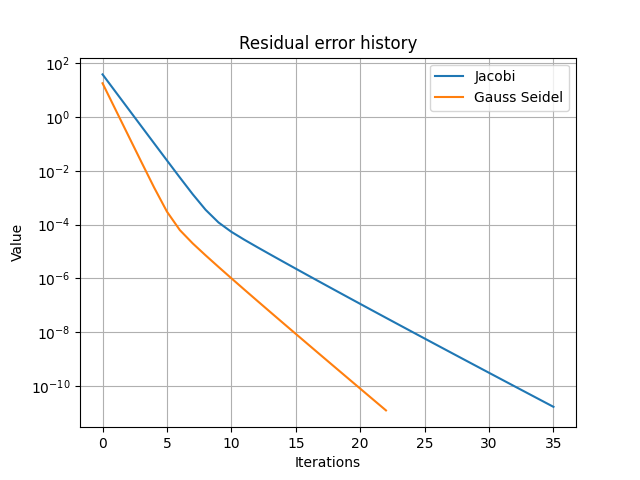
\includegraphics[width=1\linewidth]{figure0.png}
\end{figure}

\newpage
\section{Macierze nie zbieżne}
Niesty metody Jacobiego i Gaussa-Seidla nie zawsze znajdują rozwiązanie. Dla poniższego przypadku macierza pasmowego gdzie wartość na przekątnej jest mniejsza metody te zbiegają do nieskończonośći
\[
C  =
\begin{bmatrix}
3 & -1    & -1    & 0     & ...  \\
-1    & 3  & -1    & -1    & ...  \\
-1    & -1    & 3 & -1    & ...  \\        
0    & -1    & -1     & 3 & ...  \\   
...  &  ...  & ...    & ...   & ...  
\end{bmatrix}
b = 
\begin{bmatrix}
-0.75 \\
0.98 \\
-0.53 \\
-0.28 \\
... \\
\end{bmatrix}
\]
\begin{figure}[H]
    \centering
    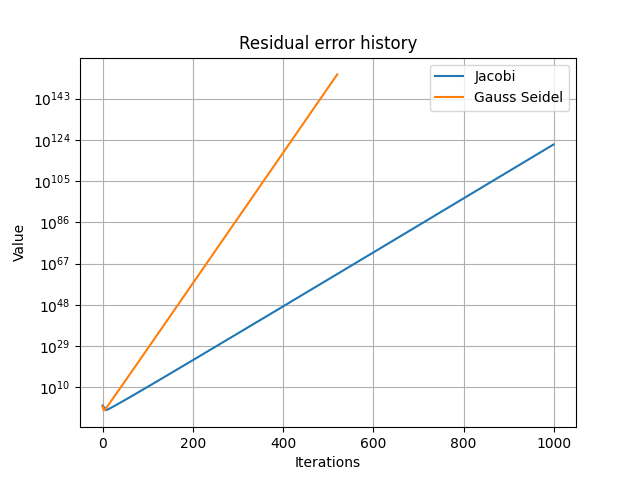
\includegraphics[width=1\linewidth]{figure1.png}
\end{figure}

Jak widać metoda Gaussa-Seidla przedwcześnie osiągneła 
wartości przekraczające zakres 64 bitowej 
liczby zmiennoprzecinkowej. 
W tym przypadku dla residum mniejszego od zera metody te nie znajdą rozwiązania. 

\newpage
\section{Metoda faktoryzacji LU}
Dla nie zbieżnych macierzy pozostaje trzecia implementacja bezpośredniego algorytmu
faktoryzacji LU. W metodzie LU macierz jest dzielony na dwa zredukowane macierze trójkątne,
z których można wyciągnąć rozwiązanie w następujący sposób. \\
\( Ly = b, Ux = y\) \\
Norma rezydualna, dla tej metody wynosi 0.0.

\section{Wydajność metod od rozmiarów macierzy}
Niestety metoda LU nie jest najbardziej wydajna, dla większych macierzy. Między innymi dlatego wymyślono metody aproksymacyjne iteracyjne o niższej złożoności obliczeniowej takie jak metoda Jakobiego i  Gaussa-Seidla.
Poniżej przedstawiono czas wykonywania, każdej z wymienionych metod.
\begin{figure}[H]
    \centering
    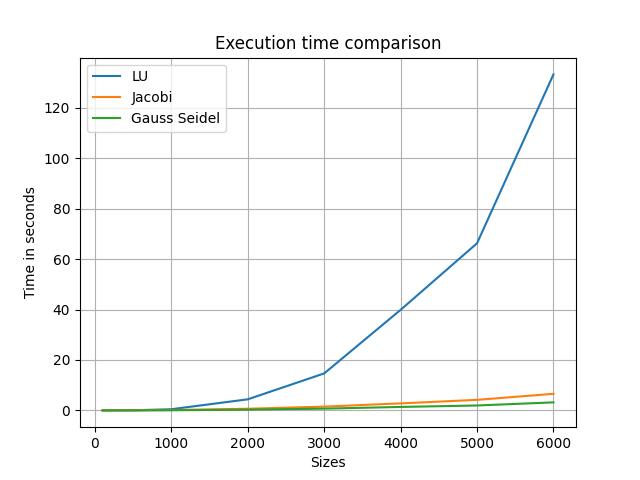
\includegraphics[width=1\linewidth]{figure2.png}
\end{figure}

Jak można zauważyć metoda LU rośnie o wiele szybciej od wymienionych metod iteracyjnych.

\section{Podsumowanie}
Metody aproksymacyjne mimo swej niedokładności są niezbędnym narzędziem do wyliczania dużych systemów równań linionych, a metody bezpośrednie jak LU sprawdzają się w sytuacjach gdy dokładność rozwiązania jest kluczowa.

\end{document}


